\subsection{Zustand: Obstalce Detouring}

Um einem Hindernis auszuweichen muss eine Router um oder vom Hindernis weg gefunden werden. Dafür prüft
sich zuerst jeder Roboter selbst, ob er am weitesten vorne im Schwarm ist, um dann als neuer Lead den 
Schwarm vom Hindernis weg zu führen. 
Zwei Kriterien müssen dafür erfüllt sein: Ein Lead darf selber nicht kollidiert sein und keinen Nachbarn
vor sich haben.
Das funktioniert wieder einfach
mittels verteilter Breitensuche. Da diese die Anzahl der Hops zur Root angibt, kann einfach ermittelt werden,
welcher Roboter am weitesten weg von einem LGP ist, um so einen Scheitel um das Objekt zu ziehen (siehe
Abbildung (a)).
Wenn mehrere Roboter den höchsten Hop zum LGP haben, wir derjenige mit der kleineren ID
gewählt. In einer Eltern-Kind-Beziehung folgen nun alle Roboter dem neuen Lead (b).\\

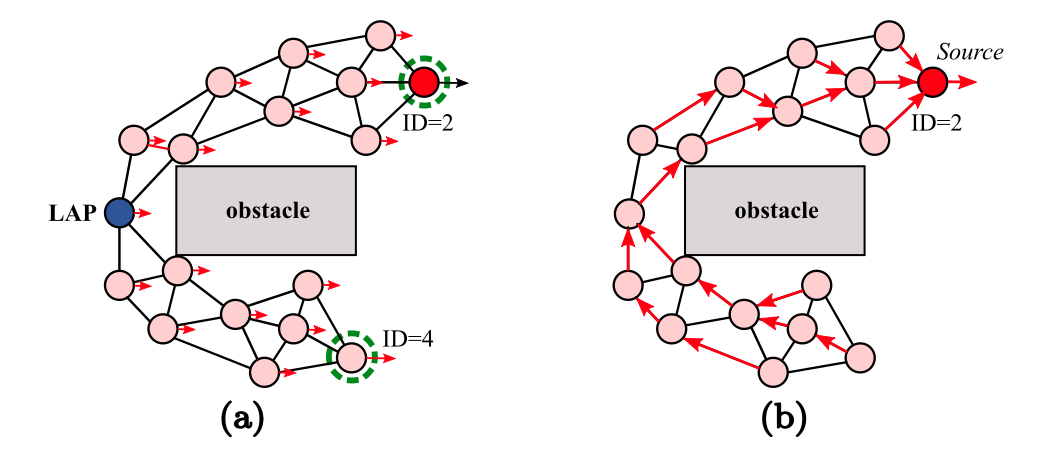
\includegraphics[width=5in]{images/Screenshot 2023-02-20 at 1.25.24 PM.png}

Dabei gilt es den maximalen
Baumwinkel, also den größten Winkel innerhalb vom Schwarm, minimal zu halten. Wenn ein vordefinierter 
Threshold für den maximalen Baumwinkel unterschritten wurde – der Schwarm also eine längliche Formation
eingenommen hat – und kein Roboter mehr kollidiert ist, geht der
Schwarm in den Reconstruction Zustand über.